\subsection{Ablation study for GCF}\label{subsec:gcf-ablation-study}
Meng Liu et. al does not present an ablation study for BiTGCF and GCF, which LightGCN showed is important with their regards to NGCF \cite{lightgcn,BiTGCF}.
In this section we conduct an ablation study on GCF to get an understanding on the effect of the different parts of the embedding propagation and layer combination.
The results can also be seen on \autoref{tab:ablation-results}, where the bold results are the best performing and underlined are the second best results.
Examples of the changed methods can be seen in the following equations.
\textit{GCF-minus-sc} can be seen on \autoref{eq:GCF-minus-sc} where the self-connection has been removed.
On \autoref{eq:GCF-only-IP} only the inner product of the neighbor has been contained, and is called \textit{GCF-only-IP}.
\autoref{eq:GCF-minus-IP} have removed the inner product and is called \textit{GCF-minus-IP}.
There are also examples where GCF utilizes summation as layer combination as used in LightGCN which can be seen on \autoref{eq:lightgcn-sum}.
The methods that use weighted summation all start with \textit{GCF-sum}.
When LightGCN is tested with concatenation as layer combination it is called \textit{LightGCN-concat}.
\begin{equation}
    \mathbf{e}_{u}^{(k+1)} = \sum^{}_{i \in \mathcal{N}_u}  \frac{1}{\sqrt{|\mathcal{N}_u||\mathcal{N}_i|}}\left( \mathbf{e}_i^{(k)} + \mathbf{e}_i^{(k)} \odot \mathbf{e}_u^{(k)} \right)
    \label{eq:GCF-minus-sc}
\end{equation}
\begin{equation}
    \mathbf{e}_{u}^{(k+1)} = \mathbf{e}_{u}^{(k)} + \sum^{}_{i \in \mathcal{N}_u}  \frac{1}{\sqrt{|\mathcal{N}_u||\mathcal{N}_i|}} \mathbf{e}_i^{(k)} \odot \mathbf{e}_u^{(k)}
    \label{eq:GCF-only-IP}
\end{equation}
\begin{equation}
    \mathbf{e}_{u}^{(k+1)} = \mathbf{e}_{u}^{(k)} + \sum^{}_{i \in \mathcal{N}_u}  \frac{1}{\sqrt{|\mathcal{N}_u||\mathcal{N}_i|}} \mathbf{e}_i^{(k)}
    \label{eq:GCF-minus-IP}
\end{equation}
\autoref{fig:GCF-NDCG-ablation-study} contains the results of the GCF ablation study for the Yelp2020 dataset, \autoref{fig:GCF-NDCG-ablation-study-amazon-cell-sport} for the Amazon-Cell-Sport dataset and \autoref{fig:GCF-NDCG-ablation-study-amazon-book} for the Amazon-Book results.
In Appendix \ref{app:recall-results-gcf-ablation} the figures of the results can be found in more detail, where the summation methods and concatenation methods are in separate figures.
All the used methods for the GCF ablation study are described in the following itemize.
The x-axis describes the every time the epochs increases by 20, and the y-axis is how well it performs regarding to NDCG or Recall.
The methods are as described here:\\
\begin{itemize}
    \item \textbf{GCF}: The original GCF method as described in \autoref{subsubsec:GCF-embed-propagation}.
    \item \textbf{GCF-minus-sc}: GCF without self connections.
    \item \textbf{GCF-only-IP}:  GCF where $e_i^{(k)}$ has been removed in \autoref{eq:GCF-embedding}, so that GCF's graph convolutions only considers the inner product of users and items.
    \item \textbf{GCF-only-IP-minus-sc}: Implemented as GCF-only-ip but without self connections.
    \item \textbf{GCF-minus-IP}: GCF where inner product has been removed.
    \item \textbf{LightGCN-concat}: LightGCN with concatenation as layer combination.
    \item \textbf{LightGCN}: Original LightGCN as described in \autoref{subsubsec:LightGCN-embed-propagation}.
    \item \textbf{LightGCN-plus-sc}: LightGCN, but with self connections.
    \item \textbf{GCF-sum-only-IP}: Implemented as GCF-only-IP except that the layer combination method used is weighted summation.
    \item \textbf{GCF-sum}: GCF where the layer combination has been changed to weighted summation instead of concatenation.
    \item \textbf{GCF-sum-minus-sc}: Implemented as GCF-sum but without self connections.
\end{itemize}
\begin{table*}[]
    \centering
    \begin{tabular}{|l|l|l|l|l|l|l|l|l|}
        \hline
                             & \multicolumn{2}{c|}{Yelp2020} & \multicolumn{2}{c|}{Amazon-Cell-Sport} & \multicolumn{2}{c|}{Amazon-Book}                                                                   \\ \hline
                             & NDCG@50                       & Recall@50                              & NDCG@50                          & Recall@50           & NDCG@50             & Recall@50           \\ \hline
        GCF                  & 0.09092                       & 0.1869                                 & \underline{0.03398}              & \underline{0.06536} & 0.04032             & 0.07035             \\ \hline
        GCF-minus-sc         & 0.09084                       & 0.1879                                 & \textbf{0.03472}                 & \textbf{0.06656}    & 0.04108             & 0.07261             \\ \hline
        GCF-minus-ip         & 0.09179                       & 0.1881                                 & 0.03197                          & 0.06294             & 0.03977             & 0.06998             \\ \hline
        GCF-only-ip          & 0.07659                       & 0.1587                                 & 0.01818                          & 0.03832             & 0.03765             & 0.06607             \\ \hline
        GCF-only-ip-minus-sc & 0.08338                       & 0.1712                                 & 0.02578                          & 0.05535             & 0.03777             & 0.06621             \\ \hline
        LightGCN-concat      & 0.0856                        & 0.1735                                 & 0.03029                          & 0.05707             & 0.03798             & 0.06519             \\ \hline
        LightGCN             & \textbf{0.1064}               & \textbf{0.2106}                        & 0.033                            & 0.06278             & \underline{0.04675} & \underline{0.08129} \\ \hline
        LightGCN-plus-sc     & \underline{0.1031}            & \underline{0.2098}                     & 0.03212                          & 0.06261             & \textbf{0.04679}    & \textbf{0.08175}    \\ \hline
        GCF-sum              & 0.09724                       & 0.1988                                 & 0.03095                          & 0.06446             & 0.04075             & 0.07205             \\ \hline
        GCF-sum-minus-sc     & 0.0956                        & 0.1962                                 & 0.03075                          & 0.0629              & 0.04114             & 0.07261             \\ \hline
        GCF-sum-only-ip      & 0.09843                       & 0.199                                  & 0.02878                          & 0.06065             & 0.04114             & 0.07212             \\ \hline
    \end{tabular}
    \caption{NDCG and Recall of the changed methods.}
    \label{tab:ablation-results}
\end{table*}

\subsubsection{Concatenation and weighted summation}
Looking at Yelp2020 and Amazon-Book on \autoref{tab:ablation-results} the methods that utilize concatenation as their layer combination method generally perform worse than the methods that utilize summation.
On \autoref{fig:GCF-NDCG-ablation-study} most concatenation methods learn faster than the summation methods, but the concatenation methods are also prone to early stopping because they start to decline in performance.
This is also the case for \autoref{fig:GCF-NDCG-ablation-study-amazon-book}, but here some concatenation methods are not prone to early stopping.
On \autoref{fig:GCF-NDCG-ablation-study-amazon-cell-sport} the methods perform differently compared to the Yelp2020 dataset.
The summation methods train for a lower number of epochs compared to the Yelp2020 dataset.
This could be because amazon cell sport is a smaller dataset than Yelp2020.
Generally it can be seen that GCF and GCF-minus-sc perform better than the other methods in \autoref{fig:GCF-NDCG-ablation-study-amazon-cell-sport}.
LightGCN performs better than the GCF methods that utilize weighted summation as their layer combination method.
However with Amazon-Cell-Sport the results vary less between the methods, although \textit{gcf-sum-only-ip} is clearly performing worse than the other methods.
\begin{figure}[]
    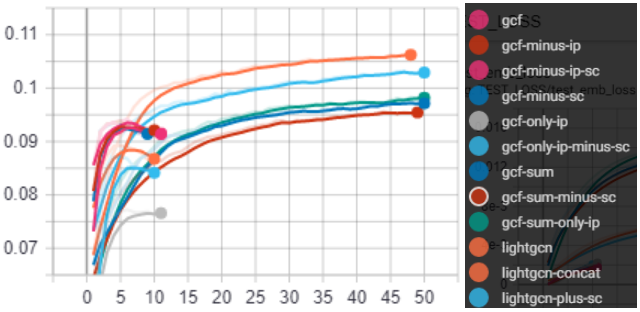
\includegraphics[width=\linewidth]{figures/gcf-all-ndcg.png}
    \caption{NDCG@50 for the Yelp2020 dataset.}
    \label{fig:GCF-NDCG-ablation-study}
\end{figure}
\begin{figure}[]
    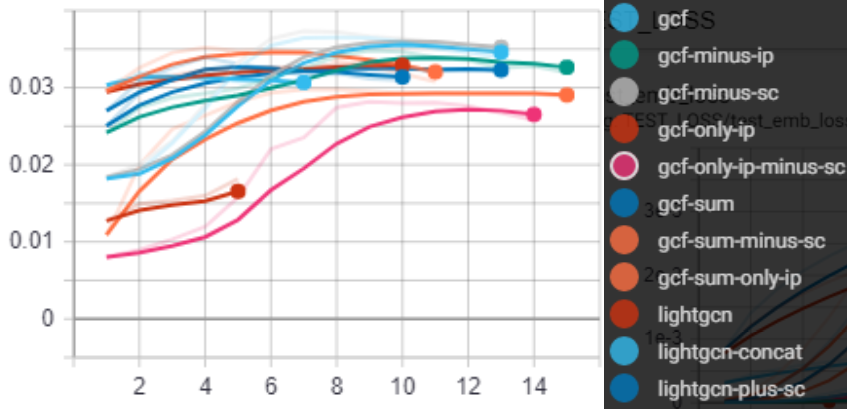
\includegraphics[width=\linewidth]{figures/amazon-cell-sport-gcf-all-ndcg.png}
    \caption{NDCG@50 for the Amazon-Sport-Cell dataset.}
    \label{fig:GCF-NDCG-ablation-study-amazon-cell-sport}
\end{figure}
\begin{figure}[]
    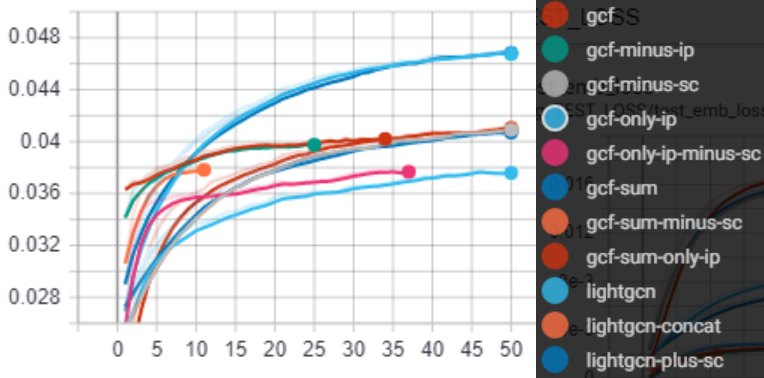
\includegraphics[width=\linewidth]{figures/amazon-book-gcf-all-ndcg.png}
    \caption{NDCG@50 for the Amazon-Book dataset.}
    \label{fig:GCF-NDCG-ablation-study-amazon-book}
\end{figure}

\subsubsection{Inner product}
Inner product makes methods using weighted summation perform worse most of the time.
The only exception is Recall@50 on Amazon-Cell-Sport for \textit{GCF-sum} which performs better than LightGCN.
This could also simply be because the inner product in general is beneficial for datasets where users or items have few connections.
For \textit{GCF} and \textit{GCF-minus-ip} it makes a small difference to add inner product in Yelp2020 and Amazon-Book, however for Amazon-Cell-Sport the method using inner product performs 3.8 \% better for Recall@50 and 6 \% better for NDCG@50.
These result can indicate that utilizing inner product is favorable when using smaller datasets.

\subsubsection{Self connections}
When comparing the counter parting methods on \autoref{tab:ablation-results} that either utilize or do not utilize self connections there is often a minimal difference on the results.
For LightGCN, GCF and GCF sum, the counterparting methods with or without self connections makes a small difference.
For \textit{LightGCN} and \textit{LightGCN-plus-sc} it varies which one performs best, but \textit{GCF-minus-sc} outperforms \textit{GCF} by a small amount most of the time.
Interestingly \textit{gcf-only-ip-minus-sc} performs significantly better than \textit{gcf-only-ip} on Yelp2020 and Amazon-Cell-Sport, which can indicate that self connections are harmful for performance, if you only use inner product in the convolutions.
However on Amazon-Book it makes a small difference.

\subsubsection{Conclusion}
The best performing methods is either GCF or LightGCN with or without self connections.
GCF is the best performing on Amazon-Cell-Sport, which is the smallest datasets, that also includes a lot of items with very few interactions.
We assume that a combination of inner product and concatenation is beneficial for learning on small datasets.
But on the larger datasets, LightGCN and LightGCN-plus-sc is the best performing methods.
